\chapter{The Matching Problem}

In the previous chapter, we saw how the system model structure can be represented in a qualitative way by using bi-partite graphs. Using this information, we need to acquire a way, ie a computation sequence, which will allow us to calculate the unknown variables in $\mathcal{X}$ from the inputs and measurements in $\mathcal{K}$. It goes without saying that such a calculation sequence cannot be derived by hand in large-scale systems. Actually, the problem of calculating each element from the set $\mathcal{X}$ using an element from $\mathcal{K_X}$ only once can be generalized to a common problem in graph theory, called \emph{the matching problem} \cite[ch~26]{Leiserson2009}.

Given a graph $G=(V,E)$, a \textbf{matching} is a subset $M\subseteq E$ such that for all vertices $v \in V$, at most one edge of $M$ is incident on $v$. We say that $v$ is matched by the matching $M$ if an edge of $M$ is incident on $v$. A \textbf{maximum matching} is a matching with maximum cardinality for a particular graph. A maximum matching is not necessarily unique. We say that a matching is complete in $V$ if $\left|M\right|=\left|V\right|$.

\section{Matchings in Bi-Partite Graphs}

In the case of a bipartite graph $G = (C,X,E)$, where $C$ is the set of constraints, $X$ the set of unknown variables and the edge set $E$ connects the variables to the constraints they appear in, the matching problem can be elaborated a bit more. For a given bi-partite graph, a matching may be complete either in $\mathcal{C}$, or in $\mathcal{X}$, or both or neither.

The following figure presents various matching for a bi-partite graph:
\begin{figure}[H]
\centering
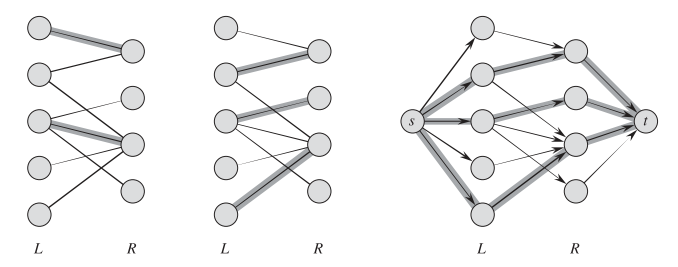
\includegraphics[width=0.7\linewidth]{Figures/matching}
\caption{Matchings on a bi-parite graph}
\label{fig:bipariteMatching}
\end{figure}

In the first and second subfigure we see incomplete matchings on the graph, both in terms of $L$ and $R$. However, the second matching is maximum, since no matching with greater cardinality can be found in this graph.

We can interpret the notion of matching for our need to solve the structural graph as follows: if a variable $x \in \mathcal{X}$ is matched with a vertex $e \in M$, then we also say that it is matched to the constraint $c \in \mathcal{C}$ which $e$ is incident onto, ie $(c,x) \in M$. This can be further extended to say that we can \textbf{calculate} $x$ by using $c$. Hence, no other variable can be calculated using $c$ and no other constraint can produce $x$.

The above interpretation applies a directionality in the bipartite graph. Let $E'$ be a new edge set where 
\begin{equation} \label{eq:matchedDirGraph}
E' = \left\{(c,x) \in E : (c,x) \in M\right\} \cup \left\{(x,c) \in E : (x,c) \notin M\right\}
\end{equation}

Through the procedure of matching, a new directed graph $G'=(C,X,E')$ is produced whose direction dictates the calculation order of the model structure and visualizes the information flow. 
\begin{itemize}
\item if an edge connects a constraint to a variable, then this variable is calculated using this constraint.
\item if an edge connects a variable to a constraint, then this variable is used by this constraint.
\end{itemize}

Paths are created, which connect variables as they contribute to the calculation of other variable, down the path.

\section{Constraints in Matchings of Graphs Representing Real-World Systems}

The matching process works very efficiently and without problems in undirected graphs. However, in bi-partite structural graphs resulting from real-world systems many problems arise, which restrict the feasibility of a complete matching in $\mathcal{X}$ and make the matching process difficult.

Notice how in (\ref{eq:matchedDirGraph}) the directionality of each edge $e \in E$ is respected. We cannot match $c$ to $x$ ($(c,x) \in M$) if $(c,x) \notin E$. Similarly, we cannot expect a variable $x$ to be used by a constraint $c$ if $(x,c) \notin E$.

Another problem arises from the fact that there is no guarantee that the calculation process created by a matching and the corresponding directional graph can be back-tracked only to known and or measured variables, ie in the transpose graph $G'\top$ there is always a path from $x \in \mathcal{X}$ to $\mathcal{K}$. This leaves us with an incomplete calculation sequence which has unknown variables as input. In the general approach, the only way to verify the feasibility of the calculation sequence is to test if $\mathcal{X}$ is \textbf{reachable} from $\mathcal{K}$ in $G'$.

Moreover, $G'$ is not guaranteed to be acyclic. The existence of cycles in $G'$ is equivalent to the presence of systems of equations in the calculation sequence which have to be solved simultaneously. Since the constraints involved are not necessarily linear and may also be differential, systems of \textbf{ordinary differential equations} or even \textbf{differential algebraic equations} may need to be solved in real-time in order for the sequence to be calculable. Depending on our assumptions, this may or may not be feasible. Initial conditions may be unknown or the mathematical and numerical tools to solve such systems may not be available to the monitoring system. Hence, we may want to mark such loops as incalculable and restrict the calculation sequence beyond them.

Finally, we may want to favour some matchings over others. Reasons to do this are to avoid too many differentiations in the calculation sequence which enhance the noise or avoid solving a constraint in terms of a variable to which the constraint has small sensitivity or high cost of implementation.

Examples for the second case are the constraints
\begin{IEEEeqnarray}{lrCl}
e_1: & x_1 + \sin x_2 &= &0 \IEEEyesnumber \IEEEyessubnumber\\
e_2: & x_1^2 + x_2 &= &0 \IEEEyessubnumber \\
e_3: & x_1 + 0.0001 x_2 + 10 x_3 &= &0 \IEEEyessubnumber
\end{IEEEeqnarray}

\begin{itemize}
\item We would prefer solving $e_1$ for $x_1$ rather than for $x_2$, since the sensitivity of $e_1$ to $x_2$ for $x_2$ around $\pi/2$ becomes 0.
\item We would prefer solving $e_2$ for $x_2$ for $x_2$ rather than from $x_1$, since calculating the power of 2 is cheaper than calculating a square root.
\item Assuming comparable variable orders of magnitude, we would prefer solving $e_3$ for $x_1$ or $x_3$ rather than for $x_2$, since $e_3$ is much more sensitive to noise in $x_1$ and $x_3$ in contrast to noise from $x_2$.
\end{itemize}

The following example demonstrates how the above constraints affect the selection of the appropriate matching.

We are given the system
\begin{IEEEeqnarray}{lrCl}
c_1: & x_1 - 100 u_1 &= &0 \IEEEyesnumber \IEEEyessubnumber\\
c_2: & 3 x_4 + 7 x_2 - x_1 + x_5 &= &0 \IEEEyessubnumber \\
c_3: & 5x_2 - x_3&= &0 \IEEEyessubnumber \\
c_4: & 10x_3 + 4x_4 &= &0 \IEEEyessubnumber \\
c_5: & x_8 - 2x_7 - x_5 &= &0 \IEEEyessubnumber \\
c_6: & x_8 - \frac{d}{dt}x_7 &= &0 \IEEEyessubnumber \\
c_7: & x_9 \cdot x_1 -1 &= &0 \IEEEyessubnumber \\
c_8: & x_6 - x_9 &= &0 \IEEEyessubnumber \\
c_9: & y_1 - \frac{d}{dt}x_9 &= &0 \IEEEyessubnumber \\
c_{10}: & x_5 - x_6^3 + 1 &= &0 \IEEEyessubnumber \\
c_{11}: & x_5 + x_1^{1.5} &= &0 \IEEEyessubnumber
\end{IEEEeqnarray}

The structural graph of the system is depicted below.

\begin{figure}[H]
\centering
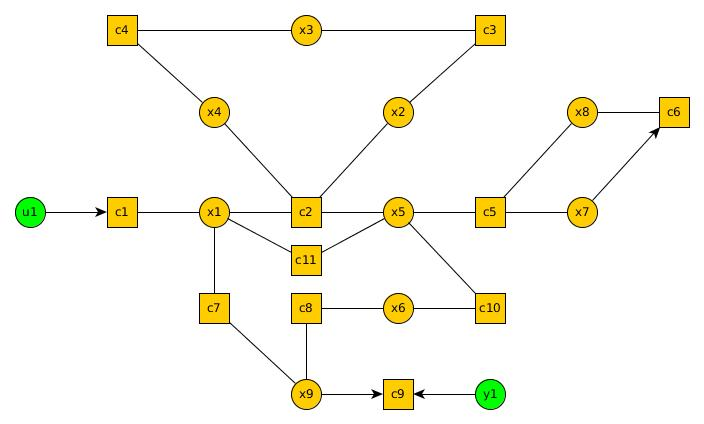
\includegraphics[width=0.7\linewidth]{Figures/unmatchedConstrGraph}
\caption{The bi-parite graph of the previous system}
\label{fig:matchingConstraints}
\end{figure}

Notice how the causality of some equations pre-enforces directionality on some of the edges:
\begin{itemize}
\item Known variables (inputs and measurements, shown in green) can only be used as inputs in the constraints, not calculated by them.
\item Variables differentiated in time can only be used as input to constraints, due to derivative causality (eg in $c_6$).
\end{itemize}

A good matching on the above graph is shown below. The edges which belong to the matching are emphasized and the rest of the edges are directed in such a way so as the matching is respected. We verify that at most one edge leaves a constraint vertex and at most one edge enters a variable vertex.

\begin{figure}[H]
\centering
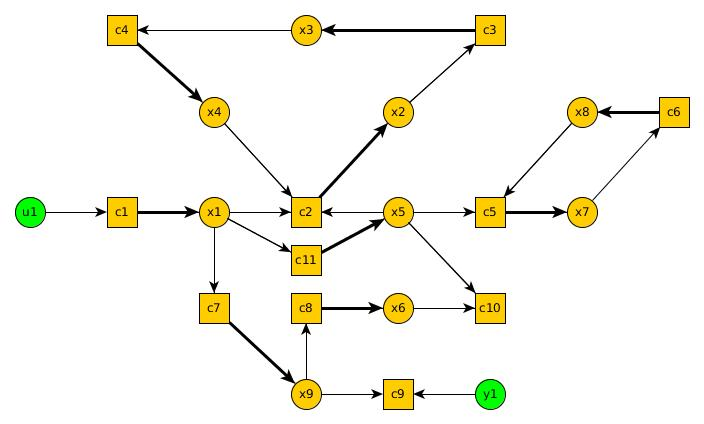
\includegraphics[width=0.7\linewidth]{Figures/matchedConstrGraph}
\caption{A matching of the structural graph with desirable properties}
\label{fig:matchingConstraints}
\end{figure}

The above matching has some very desirable properties:
\begin{itemize}
\item It is a maximum matching on the varables set.
\item The each edge of the resulting directed graph respects the directionality of the original graph.
\item When possible, the least expensive calculation is selected, as in the case of $x_6$, which is calculated through $c_8$, rather than $c_{10}$
\end{itemize}

Naturally, the existence of loops in the resulting directed graph cannot be avoided, since this is a property of this particular, actual, real-world system. Whether it is possible to solve them depends on the available analytical and numerical tools we have.